\addtocontents{toc}{\protect\setcounter{tocdepth}{0}}
\chapter*{phụ lục}\label{phuluc_intro}
\vspace{-40pt}
% --- THIẾT LẬP ĐÁNH SỐ HÌNH CHO PHỤ LỤC ---
\setcounter{figure}{0}          % Bắt đầu đếm lại từ số 0
\renewcommand{\thefigure}{\arabic{figure}} % Chỉ hiển thị số thứ tự (Hình 1)
% ------------------------------------------
\renewcommand{\thesection}{\arabic{section}} % Loại bỏ số chương (0) phía trước, chỉ hiện số thứ tự section
% Reset bộ đếm section về 0 để section tiếp theo là số 1
\setcounter{section}{0}
\section{Bổ sung 1}
\begin{figure}[htbp]
    \centering % Bỏ dấu gạch dưới ở đây
    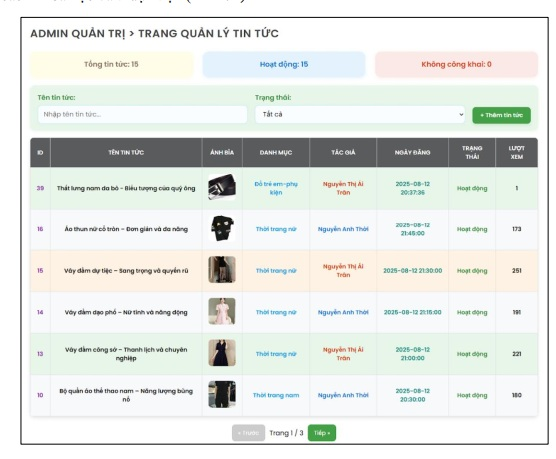
\includegraphics[width=0.7\textwidth]{Appendix/Images_phuluc/giaodientrangquanlytintuc.jpg}
    \caption[]{Giao diện trang quản lý tin tức} 
   
\end{figure}
\clearpage
\section{Bổ sung 2}
\begin{figure}[htbp] % Dùng !t để ép lên đầu trang
    \centering
    
\includegraphics[width=0.7\textwidth]{Appendix/Images_phuluc/chungnhan.jpg}
    \caption[]{Chứng nhận tri thức khoa học trẻ} 
\end{figure}

\clearpage
\section{Bổ sung 3}
\begin{figure}[htbp]
    \centering % Bỏ dấu gạch dưới ở đây
    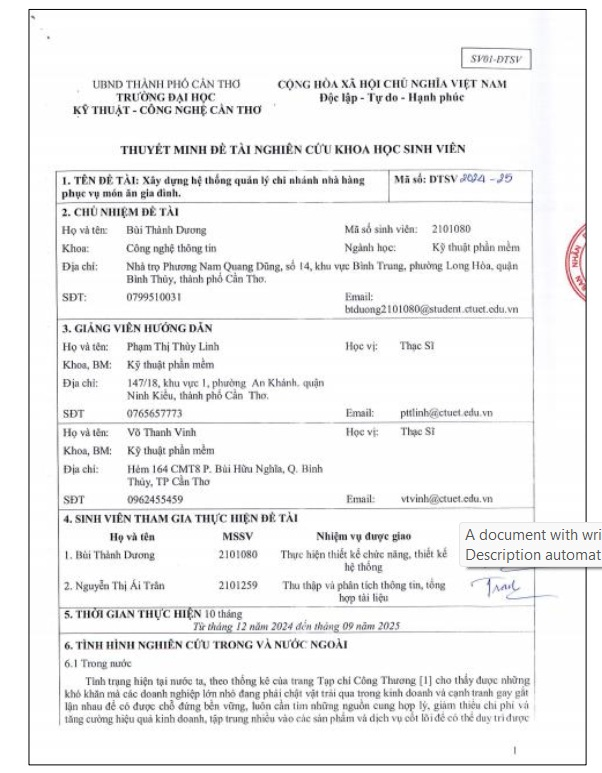
\includegraphics[width=0.7\textwidth]{Appendix/Images_phuluc/nckh.jpg}
    \caption[]{Chứng nhận nghiên cứu khoa học} 
   
\end{figure}
\clearpage